\documentclass[]{beamer}
\mode<presentation>{
  %% \usetheme[compress]{Berlin}
}
%% packages
\usepackage{zhspacing}
\zhspacing
\usepackage{graphics}
\usepackage{listings}
\lstset{basicstyle=\ttfamily\small}
\usepackage{tabularx}
\usepackage{booktabs}
%% meta info
\title{函数式并行程序语言研究}
\author[苏醒~pysuxing@gmail.com]{
\begin{tabular}{ll}
答辩人: & 苏醒 \\
指导教师: & 窦文华~教授
\end{tabular}
}
\institute{计算机所641教研室}
\date{}

%% slides
\begin{document}
\setlength{\parindent}{0pt}

\frame{\titlepage}

\frame{\tableofcontents}

\section{研究背景}
\frame{\tableofcontents[currentsection]}

%% \subsection{并行化与异构化硬件}
%% \frame{\tableofcontents[currentsection, currentsubsection]}

\begin{frame}
  \frametitle{计算硬件的发展趋势}
  \only<1>{
    单个处理器的速度已经不再继续提升…… % FIXMR: need a figure here
  }

  \only<2>{
    通过增加计算机的数量以实现更高的性能
    \begin{figure}
      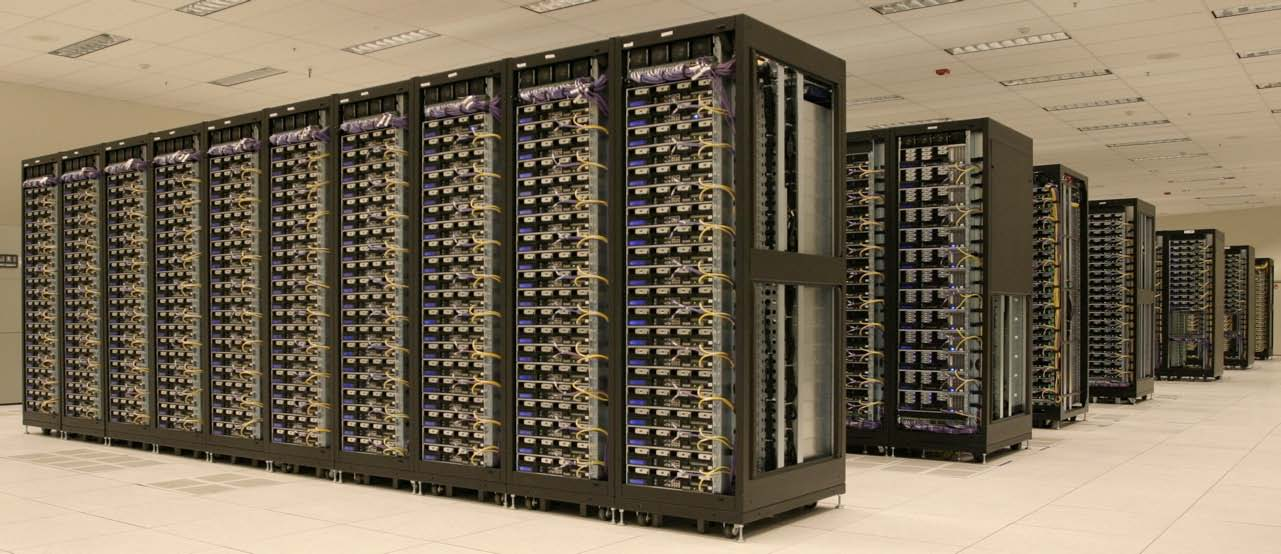
\includegraphics[height=.3\textheight]{figures/yahoo-hadoop-cluster}
    \end{figure}
  }

  \only<3>{
    为单个计算机装备多个处理器
    \begin{figure}
      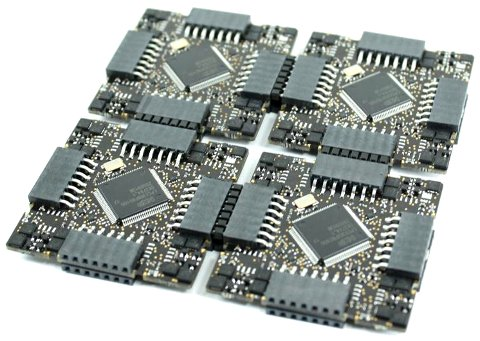
\includegraphics[height=.3\textheight]{figures/multiprocessor}
    \end{figure}
  }

  \only<4>{
    以及,在单个处理器上放置多个计算核心
    \begin{figure}
      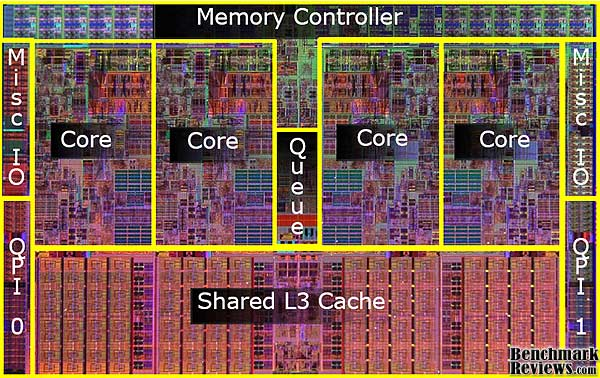
\includegraphics[height=.3\textheight]{figures/multicore}
    \end{figure}
  }

  \only<5>{
    甚至,将多个不同种类的计算设备集成到计算机系统中
    \begin{figure}
      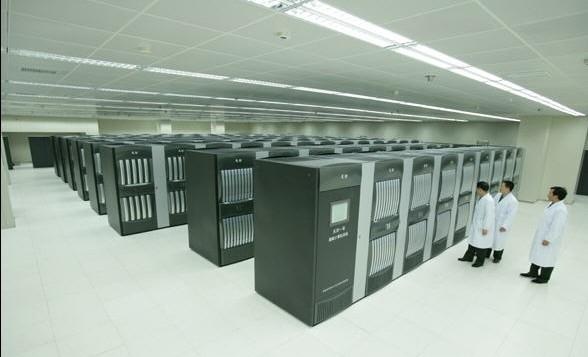
\includegraphics[height=.3\textheight]{figures/tianhe1}\hspace{1em}
      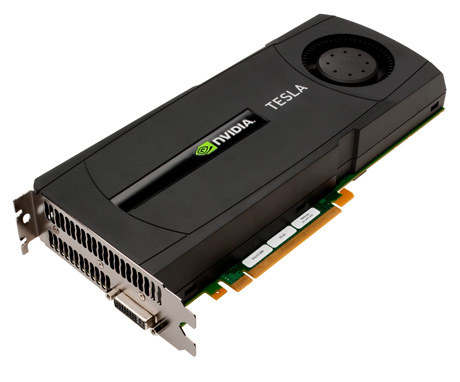
\includegraphics[height=.3\textheight]{figures/nvidia-tesla}
    \end{figure}
  }
\end{frame}

\begin{frame}
  \frametitle{计算硬件的发展趋势(续)}
  计算机系统的发展趋势
  \begin{itemize}
    \item 并行化
    \item 异构化
  \end{itemize}
\end{frame}

%% \subsection{并行软件技术}
%% \frame{\tableofcontents[currentsection, currentsubsection]}

\begin{frame}
  \frametitle{并行软件的设计目标}
  并行软件技术追求两个目标:
  \begin{itemize}
    \item 高效性\\
      以充分开发并行硬件的计算能力
    \item 易用性\\
      以提高并行程序开发效率
  \end{itemize}
\end{frame}

\begin{frame}
  \frametitle{现有并行软件技术}
  \only<1>{
    \begin{itemize}
    \item 多线(进)程---并行程序设计的基本工具
    \item MPI---在高性能计算领域的主导技术
    \item 编译制导指令(如OpenMP)
    \end{itemize}
  }
  \only<2>{
    总体上,并行编程难度远高于串行编程,编程者需要控制所有并行细节:
    \begin{itemize}
    \item 内存分配与回收
    \item 线(进)程管理
    \item 线(进)程间同步与通信
    \end{itemize}
    前述并行软件技术在高效性方面表现较好,但易用性仍显不足。
  }
\end{frame}

\begin{frame}
  \frametitle{并行程序语言}
  程序语言是人与计算机的沟通工具,并行程序语言是解决易用性问题的有力方法。
  \pause
  \begin{itemize}
    \item 专门的并行语法结构或并行操作原语
    \item 抽象层次高
    \item 细节隐藏好
  \end{itemize}
\end{frame}

\begin{frame}                   % FIXME: consider font size in this frame
  %% Rat: A {\Large FUNCTIONAL PARALLEL} Programming Language
  \centerline{Rat: 一种\ {\huge 函数式\ 并行}\ 程序语言}
\end{frame}

\begin{frame}
  \frametitle{为什么采用函数式语言设计?}
  \begin{itemize}
    \item 抽象层次高,细节隐藏能力强
    \item 高阶函数大大提高了编程灵活性
    \item 恒值对象、纯函数特性简化了程序语义,容易分析
    \item 纯函数特性使程序更容易自动并行化
  \end{itemize}
\end{frame}

\begin{frame}
  \frametitle{相关研究现状}
  \begin{itemize}
    \item Haskell语言并行技术
    \item MapReduce编程模型
  \end{itemize}
\end{frame}

\begin{frame}
  \frametitle{相关研究现状(续)}
  Haskell语言并行技术
  \begin{itemize}
    \item 并发(任务并行)
      \begin{itemize}
        \item 轻量级线程库及其操作系统线程绑定
        \item 基于策略的并行编程技术
        \item 并行 Monad
      \end{itemize}
    \item 并行(数据并行)
      \begin{itemize}
        \item Haskell 嵌套数据并行
        \item Repa: 规则数据并行
        \item Accelerates: Haskell on GPU
      \end{itemize}
  \end{itemize}
\end{frame}

\begin{frame}
  \frametitle{相关研究现状(续)}
  \only<1>{
    MapReduce编程模型:简单、有效、可扩展性强
    \begin{figure}
      \centering
      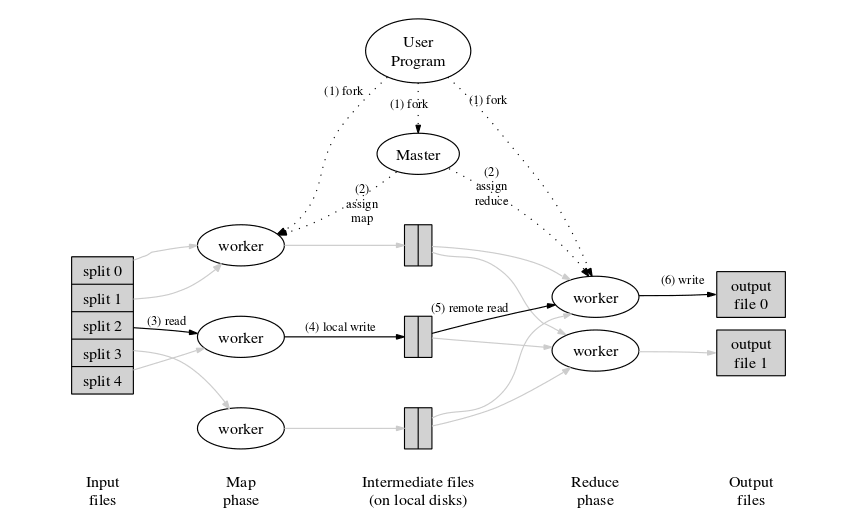
\includegraphics[height=.5\textheight]{figures/map-reduce-overview}
    \end{figure}
  }
  \only<2>{
    MapReduce实现
    \begin{itemize}
      \item 计算机集群:Google's MapReduce \& Hadoop
      \item 共享内存计算机:Phoenix:
      \item GPU:Mars \& MapCG
      \item GPU 集群:GPMR
    \end{itemize}
  }
\end{frame}

\section{研究内容}
\frame{\tableofcontents[currentsection]}
%% \begin{frame}
%%   \frametitle{研究内容}
%%   \begin{enumerate}
%%     \item 函数式语言设计
%%     \item 基于向量原语的并行编程模型
%%     \item 基于数据流的并行自动化技术
%%     \item 针对CPU/GPU异构计算机的运行时系统设计
%%   \end{enumerate}
%% \end{frame}

\subsection{函数式语言设计}
\frame{\tableofcontents[currentsection, currentsubsection]}

\begin{frame}
  \frametitle{函数式语言设计}
  \begin{itemize}
    \item “一等公民”函数
    \item 柯里化
    \item 恒值对象
    \item 纯函数特性
  \end{itemize}
\end{frame}

\begin{frame}
  \frametitle{“一等公民”(first-class citizen)}
  函数是Rat语言中的“一等公民”,即,函数可以是
  \begin{itemize}
    \item 其他函数的参数
      \lstinputlisting[language=Haskell]{listings/frag-5.hs}
    \item 函数的返回值\\
      \lstinputlisting[language=Haskell]{listings/frag-6.hs}
    \item 匿名函数(lambda表达式)\\
      \lstinputlisting[language=Haskell]{listings/frag-7.hs}
  \end{itemize}
\end{frame}

\begin{frame}
  \frametitle{柯里化(curried)}
  柯里化指函数的形式参数可以部分实例化
  \lstinputlisting[language=Haskell]{listings/frag-8.hs}

  另一种视角:可以将n元函数看作一个1元函数,该1元函数的返回值是一个(n-1)元函数
  \lstinputlisting[language=Haskell]{listings/frag-9.hs}
\end{frame}

\begin{frame}
  \frametitle{恒值对象(immutable object)}
  无赋值操作,一个对象只在被定义的时候赋值,并在之后的生命周期中不再变更
  \lstinputlisting[language=Haskell]{listings/frag-10.hs}
  %% \pause
  %% 恒值对象与纯函数特性可以大大简化程序语义的分析。
\end{frame}

\begin{frame}
  \frametitle{纯函数特性(pure functional)}
  也称“无副作用”(side-effect free),即函数的输出只依赖于它的输入参数
  \begin{itemize}
    \item 纯函数举例:\\\texttt{sqrt, pow, exp ...}
    \item 副作用函数:\\\texttt{printf, readline ...}
  \end{itemize}
  %% \pause
  %% lambda演算的理论保证了一个表达式的值与各个子表达式的求值顺序无关。
\end{frame}

\begin{frame}
  \frametitle{小结:函数式语言设计}
  为什么采用函数式语言设计?
  \begin{itemize}
    \item 抽象层次高,细节隐藏能力强
    \item 高阶函数与柯里化性质大大提高了编程灵活性
    \item 恒值对象、纯函数特性等性质简化了程序语义,容易分析
    \item 纯函数特性使程序更容易自动并行化
  \end{itemize}
  \pause                        % FIXME: use cover
  相对地,过程式(命令式)语言
  \begin{itemize}
    \item 抽象级别低,细节隐藏能力差
    \item 强迫编程者以计算机的逻辑思考问题
  \end{itemize}
\end{frame}

\subsection{基于向量原语的并行编程模型}
\frame{\tableofcontents[currentsection, currentsubsection]}

\begin{frame}
  \frametitle{Core语言}
  Core语言是Rat编译过程中的中间语言。
  \begin{figure}
    \centering
    \includegraphics[width=.8\textwidth]{figures/frontend}
    \caption{Rat编译流程}
  \end{figure}
\end{frame}

\begin{frame}
  \frametitle{Core语言(续)}
  Core语言为数据并行问题提供了一种简单灵活的并行编程模型。
  \begin{itemize}
    \item 向量原语\\
      \texttt{map, scan, gpermute, sort, ...}
    \item 标量原语\\
      \texttt{+, -, *, /, sqrt, pow, ...}
    \item 辅助指令\\
      \texttt{length, vref, if, foreach}
  \end{itemize}
\end{frame}

\begin{frame}
  \frametitle{向量原语}
  向量原语是并行数据操作的核心,在并行硬件平台上可以高效实现。
  \begin{table}
    \centering
    \footnotesize
    \begin{tabularx}{\linewidth}{cX}
      \toprule
      \textbf{向量原语} & \textbf{功能说明} \\
      \midrule
      \texttt{map} & 给定一元操作,对一个向量中所有元素施加同一操作\\
      \texttt{scan} & 给定满足结合律的二元操作,求一个向量中元素的部分和\\
      \texttt{gpermute} & 对向量中的元素重排\\
      \texttt{gcopy} & 对向量中的元素采取特定步长复制\\
      \texttt{shrink} & 对给定向量采取紧缩复制\\
      \texttt{sort} & 给定排序函数,对向量中的元素进行排序\\
      \texttt{random} & 产生随机向量\\
      \texttt{generate} & 根据位置产生向量元素\\
      \texttt{zip} & 将多个向量中的元素逐位置组成元组\\
      \bottomrule
    \end{tabularx}
  \end{table}
\end{frame}

\begin{frame}
  \only<1>{
    \begin{figure}
      \centering
      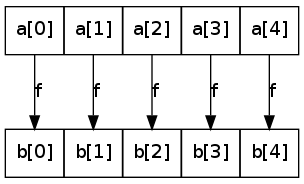
\includegraphics[height=.4\textheight]{figures/map}
      \caption{map}
    \end{figure}
  }
  \only<2>{
    \begin{figure}
      \centering
      \includegraphics[height=.4\textheight]{figures/gcopy}
      \caption{gcopy}
    \end{figure}
  }
  \only<3>{
    \begin{figure}
      \centering
      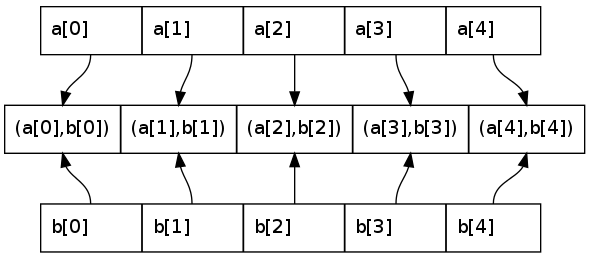
\includegraphics[height=.4\textheight]{figures/zip}
      \caption{zip}
    \end{figure}
  }
\end{frame}

\begin{frame}
  \frametitle{嵌套并行}
  通过使用高阶函数与嵌套向量类型,Rat支持嵌套并行操作。
  \lstinputlisting[language=Haskell]{listings/np-decomposition.hs}
\end{frame}

\begin{frame}
  \frametitle{实例:n-body问题}
  \lstinputlisting[language=Haskell, basicstyle=\ttfamily\scriptsize]{listings/nbody.hs}
\end{frame}

\begin{frame}
  \frametitle{小结:基于向量原语的并行编程模型}
  \begin{itemize}
    \item 受到MapReduce启发
    \item 灵活,有弹性
    \item 根据硬件设计向量原语集
  \end{itemize}
\end{frame}

\subsection{基于向量流的并行自动化技术}
\frame{\tableofcontents[currentsection, currentsubsection]}

\begin{frame}
  \frametitle{并行自动化}
  程序中存在的并行潜力:
  \begin{itemize}
    \item 向量原语操作可以在并行硬件上并行执行(硬件相关)
    \item 不存在数据依赖的向量原语操作可以并行执行(硬件无关)
  \end{itemize}
\end{frame}


\begin{frame}
  \frametitle{可并行向量操作}
  如何挖掘程序中的可并行性?
  \pause
  \begin{theorem}
    Church-Rosser定理:一个表达式的求值结果与子表达式的求值顺序无关
  \end{theorem}
  \pause
  \alert{前提:表达式无副作用!}
\end{frame}

\begin{frame}
  \frametitle{可并行向量操作(续)}
  \begin{figure}                % FIXME: part of figure could be emphasized
    \centering
    \includegraphics<1>[height=.6\textheight]{figures/n-body-core-new}
    \includegraphics<2>[height=.6\textheight]{figures/n-body-core-new-1}
    \caption{n-body问题的Core语法树}
  \end{figure}
\end{frame}

\begin{frame}
  \frametitle{向量流图}
  称施加在某个向量上的向量操作序列为程序中\emph{任务流}, % FIXME: use font size or color
  由这个向量操作序列生成的向量序列称为程序中的\emph{向量流}
  \begin{figure}
    \centering
    \includegraphics[width=.8\textwidth]{figures/frontend-stream}
    \caption{回顾:Rat编译流程}
  \end{figure}
\end{frame}

\begin{frame}
  \frametitle{向量流图(续)}
  \only<1>{
    \begin{figure}
      \centering
      \includegraphics[height=.6\textheight]{figures/n-body-core-new}
      \caption{回顾:n-body问题的Core语法树}
    \end{figure}
  }
  \only<2>{
    \begin{figure}
      \centering
      \includegraphics[height=.6\textheight]{figures/n-body-stream-new}
      \caption{n-body问题的向量流图}
    \end{figure}
  }
\end{frame}

\begin{frame}
  \frametitle{可并行向量操作(续)}
  CR定理的结论表现在向量流图中,即为:
  \begin{theorem}
    不同流的计算过程可以独立执行,他们的执行顺序不影响最终结果
  \end{theorem}
\end{frame}

\begin{frame}
  \frametitle{可并行向量操作(续)}
  \begin{figure}
    \centering
    \includegraphics<1>[height=.6\textheight]{figures/n-body-stream-new}
    \includegraphics<2>[height=.6\textheight]{figures/n-body-stream-new-1}
    \caption{回顾:n-body问题的向量流图}
  \end{figure}
\end{frame}

\begin{frame}
  \frametitle{流优化技术}
  在向量流图上进行实施两种优化措施:
  \begin{itemize}
    \item 向量原语重排(reorder)
    \item 向量原语聚合(fusion)
  \end{itemize}
\end{frame}

\begin{frame}
  \frametitle{向量原语重排}
  向量原语重排旨在交换可以换序的VP,以提高执行效率
  \lstinputlisting[language=Haskell]{listings/vp-reorder.hs}
  \begin{figure}
    \includegraphics<1>[height=.3\textheight]{figures/vp-reorder-1}
    \includegraphics<2>[height=.3\textheight]{figures/vp-reorder-2}
    \caption{实例:向量原语重排}
  \end{figure}
\end{frame}

\begin{frame}
  \frametitle{向量原语聚合}
  向量原语聚合旨在合并相邻的VP,以提高执行效率。
  \lstinputlisting[language=Haskell]{listings/vp-fusion.hs}
  \begin{figure}
    \includegraphics<1>[height=.3\textheight]{figures/vp-fusion-1}
    \includegraphics<2>[height=.3\textheight]{figures/vp-fusion-2}
    \caption{实例:向量原语聚合}
  \end{figure}
\end{frame}

%% \begin{frame}
%%   \frametitle{嵌套并行分解}
%%   通过使用高阶函数与嵌套向量类型,Rat支持嵌套并行操作。
%%   \lstinputlisting[language=Haskell]{listings/np-decomposition.hs}
%% \end{frame}

\begin{frame}
  \frametitle{向量流上的嵌套并行分解}
  \only<1>{
    \centerline{\texttt{accelerates = \alert{map} calcAccelerate cells}}
    $$\downarrow$$
    \centerline{\texttt{accelerates = \alert{foreach} cells calcAccelerate}}
  }
  \only<2>{
    \begin{figure}
      \centering
      \includegraphics[height=.6\textheight]{figures/n-body-stream-new}
      \caption{回顾:n-body问题的向量流图}
    \end{figure}
  }
  \only<3>{
    \begin{figure}
      \centering
      \includegraphics[height=.6\textheight]{figures/np-decomposition}
      \caption{嵌套并行分解}
    \end{figure}
  }
\end{frame}

\begin{frame}
  \frametitle{小结:基于向量流的并行自动化技术}
  \begin{itemize}
    \item 发掘问题无关的并行能力
    \item 高层优化技术
    \item 高度契合GPU并行编程模型
  \end{itemize}
\end{frame}

\subsection{针对CPU/GPU异构计算机的运行时系统设计}
\frame{\tableofcontents[currentsection, currentsubsection]}

\begin{frame}
  \frametitle{运行时系统总体结构}
    \begin{figure}
    \centering
    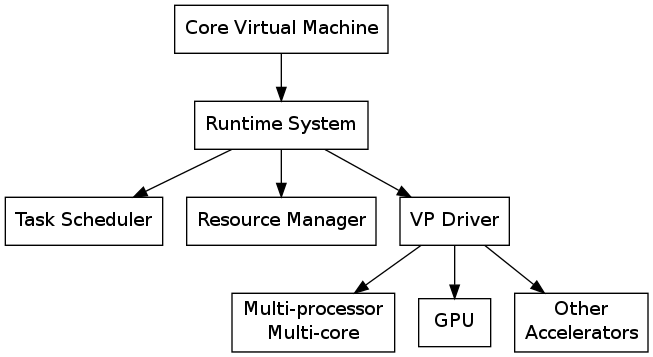
\includegraphics[width=.7\textwidth]{figures/backend}
    \caption{运行时系统总体结构}
  \end{figure}
\end{frame}

\begin{frame}
  \frametitle{任务调度器}
  GPU:任务流(stream)并发机制
  \begin{figure}
    \centering
    \includegraphics[width=.5\textwidth]{figures/stream-concurrency}
    \caption{使用stream实现并发}
  \end{figure}
\end{frame}

\begin{frame}
  \frametitle{任务调度器(续)}
  基于向量流的动态任务调度---以“单行流”为调度单位
  \begin{figure}
    \centering
    \includegraphics[height=.6\textheight]{figures/n-body-stream-new-1}
    \caption{回顾:n-body问题的向量流图}
  \end{figure}
\end{frame}

\begin{frame}
  \frametitle{内存管理器}
  向量对象的内存分布
  \begin{itemize}
    \item 向量数据位于GPU内存
    \item 元信息(长度、类型)位于CPU内存
  \end{itemize}
  \pause
  CUDA内存管理API
  \begin{itemize}
    \item 调用开销大
    \item 引入隐式同步,中断GPU计算任务
  \end{itemize}
\end{frame}

\begin{frame}
  \frametitle{内存管理器(续)}
  内存管理器:在CPU端管理GPU内存空间,采用三种内存优化技术
  \begin{itemize}
    \item 向量内存即时回收
    \item 零拷贝
    \item 向量原语原地执行
  \end{itemize}
\end{frame}

\begin{frame}
  \frametitle{向量内存即时回收}
  原理:向量对象的内存占用周期短于逻辑生命周期
  \begin{figure}
    \centering
    \includegraphics[height=.5\textheight]{figures/object-lifetime}
    \caption{向量对象生命周期与内存占用周期}
  \end{figure}
\end{frame}

\begin{frame}
  \frametitle{零拷贝}
  又称写时拷贝,指多个向量对象共享相同的内存空间

  支持零拷贝的向量原语
  \begin{itemize}
    \item \texttt{gcopy}
    \item \texttt{zip}
  \end{itemize}
\end{frame}

\begin{frame}
  \frametitle{向量原语原地执行}
  某些向量原语可以直接在输入向量的内存空间写入输出结果

  支持原地执行的向量原语
  \begin{itemize}
    \item \texttt{map}
    \item \texttt{gpermute}
    \item \texttt{random}
    \item \texttt{generate}
  \end{itemize}
\end{frame}

\begin{frame}
  \frametitle{向量原语驱动(GPU)}
  STMD编程模型:并行实现向量原语
  %% \begin{figure}
  %%   \centering
  %%   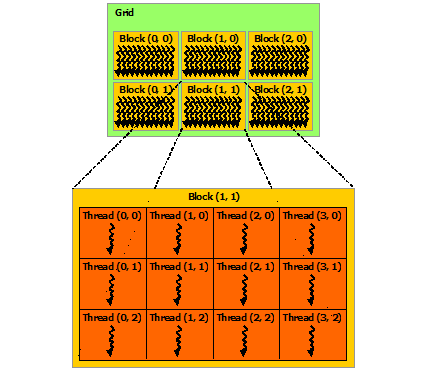
\includegraphics[height=.5\textheight]{figures/grid-of-thread-blocks}
  %%   \caption{层次化线程结构}
  %% \end{figure}
  \begin{itemize}
    \item CUDPP
    \item Thrust
  \end{itemize}
\end{frame}

\begin{frame}
  \frametitle{小结:运行时系统设计}
  \begin{itemize}
    \item 自动管理GPU内存资源
    \item 基于“单行流”的并行任务动态调度技术
    \item 向量原语的GPU实现
  \end{itemize}
\end{frame}

\frame{\tableofcontents[currentsection]}

\section{未来工作}
\frame{\tableofcontents[currentsection]}

\begin{frame}
  \frametitle{工作展望}
  \begin{itemize}
    \item 嵌套并行处理\\
      使用嵌套并行平坦化技术
    \item GPU内存\\
      内存需求总量的编译期估计,或使用渐增式内存分配策略
  \end{itemize}
\end{frame}

\begin{frame}
  \frametitle{}
  \centerline{\huge Q\&A}
\end{frame}

\end{document}
